
\chapter{Generalization Error and Model Selection }\label{ch:modelSelection}

%\section{ Model Selection}\label{section-modelSelection}


\section{Prediction and Generalization Error}\label{subsection-generalizationError}

Historically, a convenient loss function used to find the parameters was to minimize the residual sum of squares.
This measures the performance of our model $f(\cdot)$'s predictions on input samples $x$ with respect to the data\'s known output classes $y$ as

\begin{equation}
RSS(\theta_0,..,\theta_p) = \sum_{i=1}^n {[y_i - \hat{y}_i ] }^2 \\
= \sum_{i=1}^n  {[y_i - h( \theta \cdot x_i)] }^2
\label{eq:rss}
\end{equation}

% Yet this loss was favored over other functions because it is more analytically tractable and because of other statistical benefits.
% \begin{equation}\label{eq:rss}
% L(f(x),y) = \left\Vert f(x)-y \right\Vert^2_2
% \end{equation}
% When working with a linear regression with Gaussian residuals, minimizing the residual sum of squares is equal to maximizing the likelihood probability of the target, given the input data.
% This results in minimizing the following sum (RSS):
%Typical of other scenarios such as linear regression, one would like

% The equation reflects our goal to correctly match a training sample with their targets (also known as labels).

In essence, we are interested in having a generalized model, one which can make a \textit{good} prediction on any sample, even new ones from the true distribution of the data.
This generalization concept is lacking in the preceding equation because its built to fit the actual dataset which is a sample of the population.
It is not straightforward for the model to perform well with any other given sample of the \textit{true} distribution for $\mathcal{T}$.
Measuring and comparing the generalization power among models is needed to select the best supervised estimator. 
This means can be thought as correctly label new samples which wasn't used in the training phase, on independent test data from $\mathrm{T_s}$.

% We'll see why it is a bad attempt to generalize the classification model constructed from the data.
% Given that in supervised learning settings, the goal is to build a learner with low predictive error, the algorithm's generalization power will then lie on its ability to 

For now, let us assume that $f: X \rightarrow Y$ is a function which interacts the true existent relationship in the data: $Y = f(X) + \epsilon$.
In this mapping from feature to target space we also assume $\epsilon$ to be the noise, with $0$ mean and fixed $\sigma^2$ variance i.e.\ $\epsilon \sim \calN(0,1)$.
Then the equation in \cref{eq:rss} can be read as an approximation of the expected prediction error given the training set $\mathcal{T}$.


\begin{definition}{Prediction Error:}
	Given a loss function $L(\cdot,\cdot)$ and a function $f$, we say that the \textbf{prediction error} for the resulting classifier $f$ is
	\[
	PE(f_\theta)= \left[ L(\textbf{Y},f(\textbf{X}))\right]
	\]
\end{definition}

This is the error between our model transformation and the target labels, as quantified by the loss function.
 In our specific example, with the parameters $\theta$ encoding the structure of $f$ as $f_\theta(x) = h(x \cdot \theta)$ we would that that:

\begin{definition}{Squared Loss Prediction Error:}
	Given a choice of parameter $\theta$ and the \textit{squared error loss}, we say that the \textbf{prediction error} for the resulting classifier $f_\theta$ is

	\begin{equation}
	PE_{true}(\theta) =L(\textbf{y} - h(\textbf{x} \cdot \theta) )  \\
	=  {(\textbf{y} - h(\textbf{x} \cdot \theta) )}^2
	\end{equation}

\end{definition}

Our interest is now in minimizing this error for all possible values.
We would like to quantify the expected error over all random occurrences of $\textbf{X}$ and $\textbf{Y}$.
This is known as the generalization error and is very related to the prediction error as it is its expectation.

\begin{definition}{Generalization Error:}
\begin{equation}
Err = \Expect_{ \textbf{X}, \textbf{Y} } \left[ L(Y,f(X)) \right]
\end{equation}
\end{definition}

Given that any model is always built on a dataset, we are required to estimate the generalization error using only the model's error over the data available.
% $\mathcal{T_s}$:


\begin{equation}
	Err_{\mathcal{T}} = \Expect_{\textbf{X},\textbf{Y}} \left[ L(Y,\hat{f}(X)) | \mathcal{T}\right] \\
	= \int_{\mathcal{T}} {(y - h(x \cdot \theta) )}^2 P(x,y)dxdy
\end{equation}

	%\begin{equation}
	%  Err_{true}(\theta) = \Expect[(\textbf{y} - h(\textbf{x} \cdot \theta) )^2] \\
	%  = \int (y - h(x \cdot \theta) )^2 P(x,y)dxdy
	%\end{equation}

Note that in this definition the expectation is taken conditional on the training set and also from which the model is built.

%\begin{equation}
% PE = \Expect_{X,Y} \left[ L(Y,\hat{f}(X))\right] = \Expect \left[ Err_{\mathcal{T}} \right]
% \end{equation}.

In practice we have finite access to samples, so we have to estimate the generalization error.
As such, we will have data to build or \textit{train} our model.
From this reduced sample we will extract a training error to determine how well the model is performing.
This will be our approximated prediction error through the
\begin{definition}{Training Error:}
	is the average loss over the sample prediction errors:
	$$ \overline{err}_{\mathcal{T}} = \frac{1}{N} \sum_{i=1}^N L(y_i, \hat{f}(x_i) )$$
\end{definition}\label{def:trainingError}

%Let \textbf{x} $\in \mathbb{R}^{p}$ denote a random input variable and \textbf{y} $\in \mathbb{R}$ denote a random output variable with joint distribution $P\left(\textbf{x},\textbf{y}\right)$.

We will then turn to evaluate models according to their performance errors on $\mathcal{T}$ and $\mathcal{T_s}$ Combinations of high or low values for these, across training and test data, are used as model evaluation and evaluating these will point to aspects of the algorithm which need improvement.

\section{Bias and Variance}\label{section-biasVariance}

If we look closer at the generalization error in our specific case of the squared loss function with

\begin{equation}\label{squaredPE}
EPE = \Expect_X \Expect_{Y|X} \left[ \left\Vert Y - \hat{f}(X) \right\Vert_2^2 \right]
\end{equation}

It is not difficult to see that the model that minimizes this error is $\hat{f}(x) = \Expect \left[ Y | X=x \right] $.
Take Our model $\hat{f}$ to be an estimate of the true relation in the data, constructed from the data.

With the squared loss, the prediction error $\Expect \left[ \left\Vert Y - \hat{f}(X) \right\Vert_2^2 \right]$ of this model can be decomposed in the following way:

\begin{equation}\label{squaredBiasDecomposition}
\begin{split}
PE( \hat{f} ) = & {\Expect_X \left[  f(X) - \hat{f}(X) \right]}^2 + \Expect_X \left[ {\hat{f}(X)}^2 \right] \\
& - {\Expect_X \left[ \hat{f}(X) \right] }^2 + \sigma^2 \\
= & {Bias(\hat{f})}^2 + Var(\hat{f}) + \sigma^2
\end{split}
%= Bias(\hat{f})^2 + Var(\hat{f}) + \sigma^2
\end{equation}


 \cref{squaredBiasDecomposition} is hereby designated as the \textit{bias-variance decomposition for the squared loss}.
The first term is called the square of the bias of the estimator.
It measures how well off are our estimator's predictions compared to the true relational function.
On the other hand, the second and third terms are the variance of the estimator.
This will measure how this random variable varies along its most expected non-random value.
The noise's variance term is that part of the prediction error which is irreducible.
Note that we have already taken the expectation over the target and that is why we are left with the target's noise.
This part of the error we cannot minimize or control with our learner.
It is due to the random nature of the problem.

Note that here we integrate over the joint distribution of inputs and outputs.
As we've mentioned before, we have incomplete information on $P(x,y)$ given the finite data in $\mathcal{T}$.
We must assume then that calculating this integral is not possible for any $\theta$ and must rely on estimation procedures.

For example, we could try and sample $M$ i.i.d.\ points from $P(x,y)$ to approximate the integral by a Monte Carlo scheme such as

\begin{equation}\label{eq:mcarlo-approx}
Err_{true}(\theta) \approx \frac{1}{M} \sum_i^M {( y - h(x \cdot \theta) )}^2
\end{equation}

Yet this would be unfeasible as well.
Since the sampling process should be done for each specific $\theta$.
Notice however the close resemblance of the \cref{eq:mcarlo-approx} to the form in \cref{eq:rss}.

Historically the concepts of bias and variance where associated directly with the squared loss function.
 Yet in classification problems, it is uncommon to use the residual sum of squares to fit the model\'s parameters.
Instead, they rely on other \textit{loss} functions that we will introduce later.

%For this, we use a simple series approximation
%
%\begin{equation}
%Err_{train}(\theta) \approx  \Expect_{ \mathcal{T}}[{(y - h(x \cdot \theta) )}^2]
%\end{equation}

%, and can be decomposed into two types of errors

In the literature it is said that algorithms have two main sources of error, namely the bias and the variance of the learner.
And the improvement of one generally leads to a hinder on the other.
These errors are key elements in the prediction error because they point to different weak points in the algorithms.
This in turn leads to different methods to better tackle each error, where ultimately controlling both is a central to our prediction task.

Conceptually the bias error represents the model's accuracy in labeling predictions correctly.
It is the model's best attempt to capture the functional relationship among the feature and target variables.
This could either mean it is correctly assigning the sample to its correct class in classification settings, or by predicting correctly the sample's target value in a regression setting.

The bias is lower when models correctly learn the underlying structures of the data.
However, as bias decreases, the model complexity increases and more data is needed to train it correctly because the model becomes very fit to the training set i.e.\ it loses the ability to extend this predictive accuracy to new samples because they it learns too much from the available samples only.
In this situation, we have another type of error which is known as an increase in variance.

%In the generalization error, the loss function determines how \textit{good} the model's prediction are by quantifying these errors.
We can extend the notion of bias and variance to loss functions more general than the squared loss error. 
Given a training set $\mathcal{T} = (X,Y)$, let $\hat{f}(X)$ be the model's predictive function for the features and denote $L( Y,\hat{f(X)} )$ the loss function acting on the data.


%We will denote $K = |\calG|$ as the number of classes.
For the binary classification context, a common loss function used is

\begin{equation}
L(Y, \hat{f}(X)) = I(Y \neq \hat{f}(X))
\end{equation}\label{eq:classificationLossFunction}

where $Y$ will be taking any of value of the class set $\calG$.
%$$.
% In multi-class supervised problem setting,

With this, the classification prediction error can be decomposed in

\begin{equation}
Var(Y) + P(Y=\argmax_{1\leq i \leq K} P(Y=i)) - \sum_{i=1}^K P(\hat{f}(X) =i)P(Y=i)
\end{equation}

A more detailed explanation based on the works of~\cite{james-biasVarianceGeneral} is given in \cref{appx:sec:biasVarianceExtensionLoss}.

\subsection{Case of overfitting}\label{subsection-overfitting}

For any given machine learning learner, we can have a high or low variance and bias.
So there are only four possible performances of any model.
Our objective will then be to work out the data and the model to reach a state of low bias and variance.
Different states of bias and variance require strategies to make a better model.
One of the most common scenarios is having a model that has a high overall variance and low bias.

It is said in the literature that when this situation is combined with a model which gives a good performance on the $\mathrm{T}$, whilst having a poor performance on $\mathrm{Ts}$, then the model \textit{overfits} the data.
This can happen for various reasons and is mostly related to overly-complex models or having insufficient data to train, which leads to a model well trained only for $\mathrm{T}$.

Overfit models will fail to generalize on new data since the variance structure of the training set is such that the number of training samples is not enough to lower the overall variance of this model. 


% A learner with of this characteristic will only work very accurately on the train set with poor performance on new samples.
%Pero entonces todos los modelos estan overfiteados? (tomar la union de train y test?)
% This scenario is commonly known as ov \textcite{dworkFeldman-adaptiveDataAnalysis2015} defines that a learner overfits a training set $\mathcal{T}$ if it fits parameter $\hat{\theta}$ while there $\exists \theta^*$ and $\epsilon > 0 $ such that
% \begin{equation}
% Error_{train}(\hat{\theta}) < Error_{train}(\theta^*) \ and \ Error(\theta^*) + \epsilon < Error(\hat{\theta})
% %\sum_{i=0}^{\infty} a_i x^i
% \end{equation}\label{eq:overfitting}


%\todo{remove figure or do with own data.}
%
%\begin{figure}[h!]
%\begin{center}\label{figure:biasVariance}
%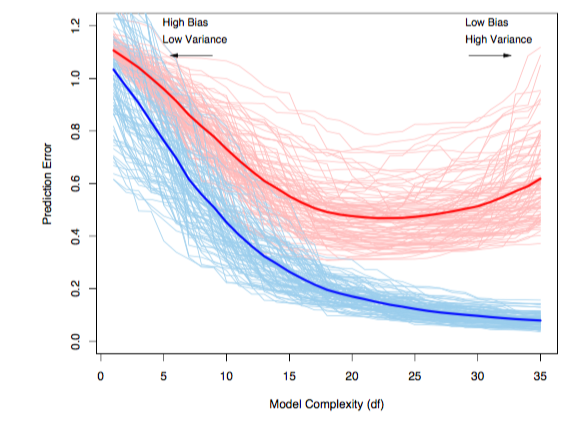
\includegraphics[width=0.7\columnwidth]{figures/figure-biasVariance/figure-biasVariance}
%\caption{ Figure borrowed from \protect\textcite{hastie-elemstatslearn} P.220.Curves are measures of the estimated prediction error for the different degrees of freedom in the model (number of features).
%Blue curves correspond to the training error and red curves are for the test error.
%The bold curves are calculated by averaging over all the colored curves.}
%
%\end{center}
%\end{figure}



To illustrate this point, in \cref{figure:dtree_overfit_problem_2} we show the results from fitting a learner on our own CDR dataset to illustrate the interaction between bias and variance.
Consider \cref{target3} which has a high imbalance between the positive and negative target classes.

Here we use a Decision Tree classifier, to try and produce a model which overfits $\mathcal{T}$.
This model can increase complexity by considering the depth of the tree.
In turn, this increases the number of features used in by the leaner to decide on the predicted target.
It is clear her that higher depth implies incresing model complexity\footnote{A detailed explanation of this technique can be found later in \cref{section:decision_trees}.}.

To score the model, we take a monotonically increasing scoring function where
higher values mean better scores.
With this, the different model errors for each complexity level, produces the following figure.

Here the test and training errors are given as a function of the tree\'s depth:

%This is because Curing the optimization procedure, the algorithm has to fit more parameters.
%In this sense, the model increases in complexity, as measured in its degrees of freedom.


\begin{figure}[h!]
\begin{center}
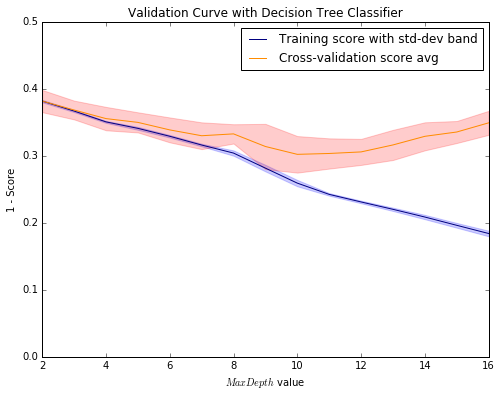
\includegraphics[width=1.2\columnwidth]{figures/figure-biasVariance/dtree_overfit_problem_2.png}
\caption{ Training and cross-validated mean score functions along the change in max tree depth.
For \cref{target2}, one model is fit for each tree depth value on both the training and cross validation sets.
Both score series are compared side by side, with their corresponding standard deviation band for the CV folds.}
\label{figure:dtree_overfit_problem_2}
\end{center}
\end{figure}


At first the model\'s bias is high both for the training and testing sets, and as a consequence, we would expect to have a high generalization error.
Then the overall error decreases as complexity increases.

The expected prediction error is shown, estimated by averaging over the test set' prediction error's.
This is seen to decrease when the model's complexity is increased.
However, when the model starts to overfit the data, the test error starts to rise whilst the train error keeps decreasing.
This situation is important to our prediction error estimation cause it hints that the model has lost predictive power due to an increase in variance.

\protect\textcite{hastie-elemstatslearn} argument that in these situations, a rough heuristic to select the best model is to stop increasing the model's complexity once the $EPE$ stops decreasing.
That is, chose the point where the scoring error of the test set stops decreasing along with the training error.
For \cref{figure:dtree_overfit_problem_2}, this would roughly be when $Max Depth = 10$.

For the examples exposed, we see that we are only finding the best model by searching only on one hyperparameter.
In practice, the models will have more parameters to tune.
This makes finding the lowest prediction error difficult.
Still, we might settle for near-optimal models which have an acceptable error score.
The following section introduces the assumptions to consider the test error as a good approximation of the generalization error.
It also gives a formal argument in favor of finding models whose scores are not optimal for that dataset.


\section{ Using the Vapnik-Chervonenkis (VC) Dimension for prediction error estimation}\label{section-VcDimension}

In Vapnik and Chervonenkis' work, the focus is put on the estimation of the prediction error through the convergence and consistency of the training error. 
To do this, the authors build a measure, the VC dimension, as an important value in determining convergence speeds for different machine learning algorithms, in the context of functional spaces. 
Here we provide only a mention of VC dimension for the purpose of showing a theoretical approach to error estimation in machine learning methods\footnote{For a complete explanation on this topic, refer to \textcite{vapnik-nature2000}}.

Vapnik-Chervonenkis propose a theoretical framework to effectively characterize these dimensions in a constructive way.
With this, they give analytic bounds to estimate the distance between the empirical error and the generalization erro for a number of machine learning algorithms.
It also provides methods to calculate these dimensions for different class of functions in a constructive way.

%since it effectively provides a tractable method to 

The Vapnik-Chervonenkis (VC) Dimension is a number based what is called \textit{Statistical Learning Theory} (SLT).
SLT is used to bound estimates the true expected prediction error from finite i.i.d.\ samples. 
Its advantage is that it requires weak assumptions from the data and the structure of the model, and the results are distribution independent. 
In addition, exact bounds are given for some common use cases with constructive analytical methods. 
For other cases, authors propose sampling or experimental methods to estimate the VC dimension. 

For this part, most of the results and reasoning follows the works in \textcite{cherkassky-learning2007}.
For a more broad development of this work, \textcite{vapnik-nature2000} is recommended too.
Here we present a brief comment on the consistency of the training error with respect to the prediction error and give example bounds for classification learners.

%In a supervised learning context, we use the empirical training ($\overline{err}$) or test errors ($\overline{err}_{test}$) to estimate the $EPE$.

Let $\mathcal {F} = \big \{ f(x,\theta) \mid x \in X, \theta \in \Theta \big \}$ be a class of classifiers where $f_\theta: X \rightarrow Y \, \forall f \in \mathcal {F}$.
This is a class of functions with domain over the input dataset $X$ and which are indexed by a parameter $theta$.
%This parameter will represent the index over the functions in $F$ and it will vary over all possible models attainable by our algorithm.

As an example, in logistic regression, $theta$ can be indexed by the values of each feature's weights $x^p$.
The class $F$ will then represent the set of all possible functions from which to select the optimal model.
%In applications, a learner is fit from a class of functions.

As it was seen before in \cref{ch:machineLearning}, a common problem in supervised learning when a particular learner is fit and then used to predict new values is overfitting.
In practice, this is common when $n$ is \textit{small} or when the number of features is \textit{large}.

Incorporating the loss functions directly into the model, SLT looks at functions of the form $Q(t,\theta) \ = \ L(f_\theta(x,y))$.
Seen as a two variable function where $t=(x,y)$ represents a sample of input and output data expressed as a random variable.%, and $theta$ the class index.

In this way, the $EPE(\theta)$ for any model takes the functional form


\begin{equation}
\begin{split}
EPE(\theta) = & \ \Expect_{\textbf{t}} \left[ Q(t,\theta) \right]\\
= & \int Q(t,\theta) p(t) dt \\
= & \int L(f_\theta(x),y) p(x,y) dx dy
\end{split}
\end{equation}\label{eq:vapnik-risk}

where we let $p(t)$ be the \textbf{true} underlying probability function of the data.
For simplicity, in this analysis we will assume the functions $Q$ in the class to be bounded.

%SLT theory then focuses on functions which seek to minimize a certain functional characterized by the form of the loss function.
Knowing that we only have access to restricted data, we would like to estimate the risk functional for that functional space, only with the available information given by training and test errors.
In this framework, this is called the empirical risk:

\begin{equation}\label{vapnik-empiricalRisk}
Err_{train}(\theta) = \sum_{i=1}^n Q(t_i,\theta)
\end{equation}

Note that the learner is estimated directly through the risk functional, which in turn is shaped by the loss function.
%The loss function is placed together with the approximating function and takes a strong part in the minimization procedure.
On the other hand, the unknown true underlying distribution $p(t)$ will not be estimated to minimize the functional and SLT puts focus in using the training error as a \textit{good} substitute for the prediction error.


%We know that the training error depends on the model learned from the data and in turn, this depends on the sample.
%Due to this non-deterministic aspect of the problem, we will have different output models for varying input samples, and even sometimes for the same sample.
%and $\theta^{*}_n$


\begin{definition}{Consistency of the Training error}

As a principal characteristic of SLT, we have that if we increase the sample size, we would still want to have the training error converge and to be consistent with the prediction error of the models.

More specifically, let $\{\mathcal {T}_1, \mathcal {T}_2, \ldots, \mathcal {T}_n, \ldots \}$ be a set of training samples such that $\forall n \ |T_n|=n$.
Given a training sample of size $n$ and a class of learners $\Theta$, let $\theta^{*}_n$ be the argument minimizing the training error and let $\theta_0$ be the minimizing argument for the prediction error over the class of functions i.e.\ over all the models of this class.

Then, the training error is said to be consistent if

\begin{equation}
\lim_{n\to\infty} Err_{train}(\theta^{*}_n) \ = \lim_{n\to\infty} EPE(\theta^{*}_n) \ = EPE(\theta_0)
\end{equation}

\end{definition}

The property of asymptotic convergence in the training and prediction errors is expected for any learning algorithm.
In SLT, the consistency requires that the training and prediction errors' sequences not only converge to the same values, but that the sequence of minimal training errors also converge, to the minimizing value of the prediction error.
%At the same time, the sequence of prediction errors must converge to this same point.

In reality, it is reasonable to think that the approximation of the prediction error with the training error introduces a strong overestimation.
The training error will also be biased by the sample used whilst the prediction error, which is given for the whole class, is not dependent on the sample.
This is very important, since the minimization of the training error when using bounded loss functions is consistent if and only if:

%\begin{definition}{Uniform Consistency of the Training Error}

%\end{definition}
\begin{equation}
\forall \epsilon > 0 \ , \ \lim_{n\to\infty} P\left[ \sup_{\theta \in \Theta} \mid Err^{n}_{train}(\theta) - EPE(\theta) \mid  > \epsilon  \right] = 0
\end{equation}

Here the training error $Err^{n}_{train}(\theta)$ is the value of this error when using a sample of size $n$.
In this sense, the training error is said to be consistent if it converges uniformly in probability over the whole class of functions\footnote{Remember that approximating functions in the SLT setting are indexed by the $\theta$ parameter.}.
This implies that the capacity of the learner will be captured in the set of functions $Q(t,\theta)$ used to approximate the data. 

%will be important in finding an appropriate model. SLT theory then introduces

	Four our work in binary classification, the main results of the VC theory establish that, for any given $\epsilon > 0$ 
\begin{equation}
P\Bigg(  \left|  Err^n_{train}(\theta^*) - EPE(\theta_0) \right| > \epsilon \Bigg)  \leq 8 poly(\Theta,n) \exp{\large \left( {\frac{-n\epsilon^2}{32}} \right)  } 
\end{equation}\label{eq:vapnik-binaryBoundProbability}

where $poly(\Theta,n)$ is a polynomial on $n$ whose coefficients depend only on the class of functions $\Theta$, through the VC dimension value. For a longer list of results of the VC theory concerning prediction error bounds for binary classifiers, see \cref{appx:sec:vcDimension}.

For practical applications though, use of these bound estimates might be limited to the determination of the VC value. This becomes increasingly difficult in algorithms which are more complex and expressive, such as neural networks. 
Due to this limitation, we show in the next section a practiced approach which is an easier and direct heuristic used to estimate the $PE$.



\section{Cross Validation}\label{section:crossValidation}

Classification models are algorithms which build approximating functions to a stochastic process, by means of algorithms. Due to the searching nature of this process, in the generally large space of hyper-parameters, we have that when models are fitted, we end producing different learners. 
 
These differences between learners are controlled by the \textit{parameters} or configuration of the algorithm. 
And each parameter's nature can appear either from computational or statistical variations to the algorithm.
An example of this, which was introduced in \cref{section-hyperParametersRegularization}, is the $\lambda$ penalization parameter in logistic regressions. 
Here, $\lambda$ controls the amount of weight to be placed on the regularization term of the minimized function.

To help in this process by means of better estimating the $EPE$, Cross Validation is a technique introduced to systematically explore tuning parameters values and decide which learner is better for the task at hand. 
By comparing the generalization error of each model, where models vary accordingly with the values of the hyper-parameters, an evaluation value is produced and used to select the \textit{best} model in the class.

This technique is considered one of the most widespread to evaluate the generalization performance in a set of learners.
Given a number of possible configurations or values for the tuning (hyper) parameters of an algorithm, we would want to decide which selection of these fit the best estimator $\hat{f}$, as measured by the generalization error.

%
%In terms of the concepts introduced before, the quality of an estimated model  from a family of algorithms is evaluated in the Cross Validation procedure.
%Where quality refers to the rate of generalization error.

In most problems we will have that data is scarce.
At the same time, the prediction error estimates are based on asymptotic or analytical results which are hardly computable in practice. 
Thus CV intends to prevent over-fitting by iteratively holding out a random part of the dataset and by measuring the predictive accuracy of the learner fit of data \textit{in-sample} against values from the \textit{hold-out} part of the dataset. 
In a sense, hold-out samples are ``new'' to the learner. 
As usual, the evaluation measure here is given by the loss function, which we must select beforehand.

\subsection{Cross Validation (CV) Procedure}\label{subsection:crossValidationProcedure}

In this method, a partition of the samples is called a \textit{fold}.
CV will then partition the data into $K$ random separate \textit{folds}, where the number $K$ has been preset\footnote{ We assume here that we are selecting samples from the training set $\mathcal{T}$ and not from the test set $\mathcal{T_s}$.}. 

Let $\gamma : \{1,..,N\} \mapsto \{1, .., K\}$ be a function mapping samples to folds.
Without loss of generality, let $\alpha$ be an index of the model's hyper-parameters configurations, where each distinct value combination of the tuning parameters is identified by this index\footnote{ Note that the domain of $\alpha$ will vary with each model, which defines the type of algorithm used to learn.}. 

The CV algorithm now runs iterations over all the folds, and takes one fold $\gamma^{-1}(\{k\})$ to be the validation set, where $k \in [1,\ldots,K]$ is the iteration indexer. 
We also have that $\hat{f}^{-k}$ denotes the fitted estimator on the training set, with the $k$-fold hold out. 
Its classification performance will be tested against this \textit{out of sample} estimates. 
So we will have that for every sample in this $k$-fold, we measure the loss $L(y_i, \hat{f}^{-\gamma(i)}(x_i))$ of the model's prediction against the true target's value. 

Cross validation intends to estimate the expected \textit{out-of-sample} error $\Expect \left[ L(Y, \hat{f}(X)) \right]$, when the model is tested against \textbf{independent} samples from the true distribution.
For this reason, it is fundamental to ensure independence of the training set and the test set.
Any data transformations that must be done on the input data $X$ that jointly uses the output samples $Y$ in the process, must be done or ``learned'' only on the training set. 
This is because we must not introduce information from our test set into the final estimator. 
The model has to be agnostic to any information contained in $\mathcal{T_s}$.
In a sense this means that the learner never ``sees'' any test data until we use it to evaluate our learner's performance.

\subsection{Selection of tuning-parameters (hyper-parameters) }\label{subsection:selection_hyper_params}

 Let $\mathcal{A} = [\alpha_0, \alpha_1,\ldots, \alpha_l  ]$ be a list of hyperparameter settings and $\mathcal{K} =[1,..,K]$ a list of folds.
A full K-Fold Cross Validation pseudo algorithm takes the following form.

 \begin{algorithm}[H]
 \KwData{All hyper-parameter configurations $\mathcal{A} = [\alpha_0, \alpha_1,\ldots, \alpha_l]$ and a number $K$ of folds.}
 \SetAlgoLined\KwResult{Data table mapping error scores to hyper-parameter configurations $CV(\alpha) \ \forall \alpha \in \mathcal{A} $}
 Initialize $\mathcal{A}$ and $\gamma(\cdot)$\;
 \For{ $\alpha \in \mathcal{A}$}{
 \If{data transformation}{
 Perform data transformation on the whole training set $\mathcal{T}$ \;
									 }
 \For{ $k \in \mathcal{K}$}{
 	 \If{feature selection}{
 	 	Perform feature selection on the $\textrm(T)^{-k}$ \;
 	 }
 fit $\hat{f}^{-k}(\cdot, \alpha)$\;
										}
 compute $CV(\alpha) = \frac{1}{N} \sum^n_{i=1} L\left( y_i, \hat{f}^{-\gamma(i)}(x_i, \alpha) \right)$\;
												}
 \caption{Pseudo-algorithm for K-Fold Cross Validation Estimation for an index of $\alpha$ hyper parameters.}
 \end{algorithm}

Note that during the loop for $\alpha$, each sample's prediction is tested on the model which was fitted without using that same sample.
This is central to the idea of cross-validation in which training samples are used \textit{as if} they were testing samples.
Samples that are not used to train the model in the CV procedure are called validation samples.

With this method, it makes sense to choose a final model $\hat{f}_\alpha$ with the lowest $CV(\alpha)$ value among all possible hyper-parameters.
However, following ideas detailed in \cref{section-VcDimension}, importance should also be given to the \textit{complexity} of the approximating function.
A common rule of thumb is to favor models in which we use a lower number of hyper parameters or number of features.
In practice however, a class of approximating functions might have a defined complexity which is not analytically computable.
Thus in some cases, crude heuristic estimates or common sense is used to estimate model complexity, without making use of theoretical arguments.


\subsection{CV run on CDR data}\label{subsection:cvExperiment}

As an example, we consider here a cross validation procedure over a logistic regression model, using for \cref{target2}.
The hyperparameter we decide to optimize is the regularization of the model as $C = \frac{1}{\lambda}$. 
We are trying to find those users that used to live in the endemic area and migrated. 
Recall from \cref{eq:logitRegularization} that this is the regularization strength of the model, where a smaller value in $C$ meant a stronger regularization.
We perform this experiment and consider the difference in scores between  $\mathcal{T}$ and $\mathcal{T_s}$ along each value.
It is important to note that all test scores were performed on models built only from $\mathcal{T}$.


\begin{figure}[h!]
\begin{center}
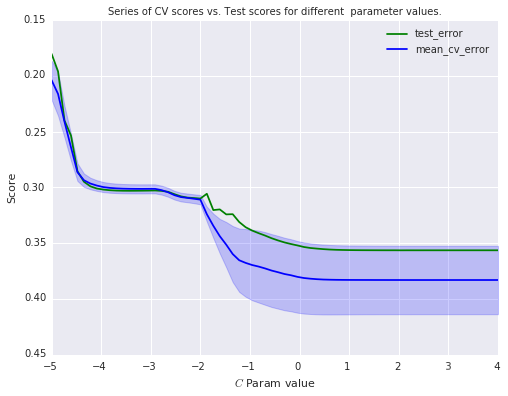
\includegraphics[width=1.2\columnwidth]{figures/cross_validation/train_and_cv_score_comparison_logreg.jpg}
\caption{ Comparison of 12-fold cross validated and test average errors for \cref{target2}.   $1-NLL$ scores are shown for each value of the regularization parameter $C$. Standard deviation bands on the $K$ fold errors are added to the CV series.}
\label{fig:cv_vs_test_score}
\end{center}
\end{figure}

In \cref{fig:cv_vs_test_score} the x-axis carries the parameter $C$'s values on a log scale. 
The score used is the negative log loss function on a twelve fold cross validation set, as well as a test set. 
It is interesting to see that for low $C$ values, the test and CV scores are very similar. 
This is probably due to the fact that being on a log scale, the regularization dominates the optimization routine.
However, at some point near $\exp^{-4}$, both lines separate differ in a notorious way.
This continues to be notorious in the direction of increasing $C$ values.
Here it can be seen that the test score is barely in the one standard deviation band of the average CV score.
This image serves as an example of how different the CV and test scores can be. 


With this we have come to show an example of how Cross Validation approximates the test error of a model.
The method required only minimal information from the data to do this, yet we have to preset a value for the number of $K$ folds to use. 

To determine this value a priori might not be possible and experimental results in the literature show the different results for CV routines with varying $K$ number of folds. 
For more information on this please refer to \cref{appx:sec:optimalKfoldNumber}.


\subsection{CV Scores in Classification Learning}\label{section:scoring_functions}

In binary classification, the contingency table summarizes all the learner's training performance for all samples in $\mathcal{T}$. 
We have that for each sample, there can only be four possibilities when comparing the model's prediction and that sample's observed target value.
The contingency table then shows the count of the amount of samples that fall into one of the these four groups. 

Let $\hat{f}$ be our model learned from the data after a CV procedure.
Every sample has a target value $y$ and a predicted outcome $\hat{y}$ and there are only four possible interactions of these two variables, for two binary outcomes each.
We can express the models' target value $\hat{y}$ into the positive ($\hat{P}$) or negative ($\hat{N}$) categories. 
At the same time we can set actual target data into the positive ($P$) or negative ($N$) categories.

To assess the performance of the classification algorithm and pick the \textit{best} model we must decide on how the CV procedure will value two different models.
We must evaluate the mismatch between the target and the predicted value in a quantifiable way.
Here loss functions are also known as \textit{scores} or \textit{measures} and are built by looking at how many times an algorithm misclassified instances, and where is the misclassification happening.
To visualize this, the \textit{confusion} table presents these results in the following draft:

\noindent
\renewcommand\arraystretch{1.5}
\setlength\tabcolsep{0pt}
\begin{tabular}{c >{\bfseries}r @{\hspace{0.7em}}c @{\hspace{0.4em}}c @{\hspace{0.7em}}l}
\multirow{10}{*}{\parbox{1.1cm}{\bfseries\raggedleft\ Target\\ value $y$}} &
& \multicolumn{2}{c}{\bfseries Predictive value $\hat{y}$} & \\
& & \bfseries \^{P} \ $(0)$ & \bfseries \^{N} \ $(1)$  \\
& P \ $(0)$ & \MyBox{True}{Positive (TP)} & \MyBox{False}{Negative (FN)} & \\[2.4em]
& N \ $(1)$ & \MyBox{False}{Positive (FP)} & \MyBox{True}{Negative (TN)} & \\
%& total & P \ $(0)$ & &
\end{tabular}

These cell values count the amount of instances that fall into each of the four possible outcomes.
Building from this, we have metrics scores constructed to provide values on the algorithm's performance. 
These counts are combined in different transformations in order to measure varied aspects of an algorithm's classification performance.

Some of the most common metrics include the following:

\begin{itemize}
\item \textbf{True Positive Rate (Recall):} $\frac{TP}{P} = \frac{TP}{TP + FN}$ \\ This rate measures the percentage of real positive values captured by the algorithm.
A high recall of the algorithm indicates that a high number of the real positive labels were classified as positive.


\item \textbf{Positive Predictive Value (Precision):} $\frac{TP}{\hat{P}} = \frac{TP}{TP + FP}$ \\ This rate measures the \textit{confidence} of the algorithm in its positive predictions, where a high precision indicates value in its predictions.

\item \textbf{True Negative Rate (Specificity):} $ SPC = \frac{TN}{N} = \frac{TN}{TN + FP}$ \\ This rate measures the percentage of real negative values captured by the algorithm.


\item \textbf{False Positive Rate (Fall-Out):} $FPR = 1 - SPC$ \\ This rate measures the percentage of false negative values misclassified by the algorithm.

\item \textbf{Accuracy:} $\frac{TP + TN}{P + N} = \frac{TP + TN}{TP + FP + TN + FN}$ \\ This rate measures the \textit{confidence} of the algorithm in all of its predictions.


\item \textbf{F1 Score:} $\frac{TP + TN}{P + N} = \frac{TP}{TP + FP} = 2 \frac{1}{ \frac{1}{recall} + \frac{1}{precision} }$ \\ This is the harmonic mean of the recall and the precision METRICS.\@ It's advantage is that it can capture both of the scores in equal weight.
Its values range in the ${[0,1 ]}$ domain and are ordered in the sense that perfect classifiers have an $F1$ score of 1.

\end{itemize}


To illustrate the difference in these metrics we ran an experiment on \cref{target2}.
We took one logistic classifier with common settings and we ran a cross validation procedure over values of the regularization strength $C$.

In this run, we considered four metrics to cross-validate our models: $Accuracy$, $Precision$, $Recall$ and $F1$.
We compared all of them in a procedure which had fixed hyper parameters for all models.
The value of folds $K$ was set to eight and the the $l1$ regularization value was optimized. 
At the same time, we fixed to 100 the maximum gradient descent iterations in any iteration. 
We also balanced the positive and negative classes in the loss function, where samples of the under-represented class had a higher contribution to the loss.
This weight was equivalent to the reciprocal of their ratio in the total count of samples.

For each metric, the best model output from the CV procedure which was selected based on the score. 
All winning models were then evaluated against $\mathcal{Ts}$ to give a final evaluation metric on the model's performance.
No other information from $\mathcal{Ts}$ was used during the whole process.
In \cref{tab:metrics_comparison_logreg_target1_results} shows a summary of these benchmarks.


\begin{table}[!htb]
\caption{ Results comparing an 8-fold CV fit of a Logistic Classifier over varying regularization $C$ values.
Four metrics were cross-validated and compared in this experiment: $Accuracy$, $Precision$, $Recall$ and $F1$.}
\label{tab:metrics_comparison_logreg_target1_results}
\centering
\begin{tabular*}{0.9\textwidth}{@{\extracolsep{\fill} }  l l l l l }
%{|p{2cm}|p{2cm}|p{1.5cm}|p{1cm}|p{1.5cm}}
\toprule
Metric & Best CV $C$ value & Mean CV score & Test score & Full CV time (s)  \\
\midrule
$Accuracy$ & 3.162 & 0.685 & 0.695 & 4628.3  \\
$Precision$ & 0.107 & 0.242 & 0.232 & 4638.2 \\
$Recall$ & 0.0006 & 0.673 & 0.668 & 4667.5 \\
$F1$ & 0.0015 & 0.339 & 0.340 & 4612.1 \\
\bottomrule
\end{tabular*}
\end{table}

It is clear from these results  that there are no significant time differences in choosing one metric over another. 
Added to this, all metrics favor stronger regularized models, except for the $Accuracy$ metric which favored a very loosely regularized model in the CV procedure.
The biggest difference between the test and average CV scores among all models was of 4\% yet still the algorithm has trouble finding samples of the positive class.
This is evidenced in the extremely low value for the $Precision$ scores where only a handful of positive classes can be correctly captured by the model.
The effect of the low precision is also evident in the $F1$ score which drags this metric down, even when the recall is has an acceptable rate of 0.65.
In practice, the experimenter would chose the metric which would be most appropriate for the task at hand.
Then, the quality of solutions vary in the way they are evaluated and this evaluation will depend on the task.


\subsection{ROC Curve}\label{sub:roc_curve}

One last important metric commonly used in classification tasks is the \textbf{Area under ROC curve (ROC AUC)}.
This metric applies only to algorithms which output for each sample the probability of belonging to the positive class.

With these algorithms we would have that the output label will be defined as

\begin{equation}
\hat{y} =
\begin{cases}
&1 \ \mbox{if} \ f(x) > \pi \\
&0 \ \mbox{else}.
\end{cases}
\end{equation}

where $\pi$ is a threshold value which will separate positive from negative samples.


If we consider different values for $\pi$, we will see that the recall $R$ and the fall-out $FPR$ of the algorithm will vary accordingly.
With this, we can define the ROC curve to be

\begin{equation}
\sigma(\pi) = (R_\pi, FPR_\pi)
\end{equation}

As expected, there exists an inverse relationship between these two as the threshold is varied.
The image of $\sigma(\cdot)$ is a curve defined in $[0,1]\times[0,1]$ which is referred to as the \textit{ROC space}.

To find a balance between these two rates, the ROC AUC metric measures the integral of this curve in ROC space.
The score calculated is thus known as \textit{Area Under the ROC Curve}.

This metric follows the same properties as the ones mentioned before, where the best classifiers have values nearer to $1$.\footnote{As a side note, the ROC AUC measure is proportional to the statistic of the Mann-Whitney U-test, where the means of the classifier's output positive and negative classes are compared.
More information on this can be found in \textcite{mason-rocAucRelationship}.}

The following figures are example ROC curves for two of the problems defined from our dataset.

\begin{figure}[h!]
\begin{center}
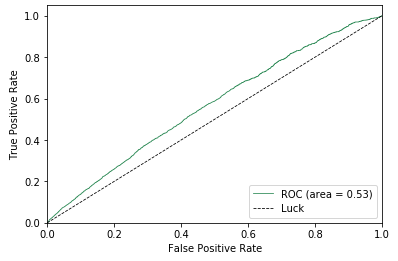
\includegraphics[width=1.2\columnwidth]{figures/figure-lowROCAUC/figure-lowROCAUC_original}
\caption{Example of a ROC curve from a Decision Tree classifier used on \cref{target2}. A 8-fold CV procedure is fit and then the best learner's performance is evaluated on $\mathcal{T_s}$ which gives score of $0.53$. This model was specifically grown to overfit the dataset by growing a tree of 12 levels.}
\label{fg:lowROCAUC}
\end{center}
\end{figure}

Notice the algorithm's poor prediction performance where the ROC AUC is near to the `luck' line.
This line constitutes the performance of a \textit{random} classifier which arbitrarily labels samples as being to each possible class.
It is expected to see good learners have better ROC AUC scores than the \textit{random classifier}.
To do this fit, we configured a very limited search over the Tree's hyper-parameters.
This, as shown, output a model which did not optimize the generalization error. 


As a counter example, another algorithm was run on the same data as in \cref{fg:lowROCAUC}, yet on a different problem.
In this case the result is that the algorithm has a considerable better score by the ROC AUC metric.
No data transformation has been applied to the set between runs.
The difference in the two scores is notable and corresponds entirely to the problem chosen.

\begin{figure}[h!]
\begin{center}
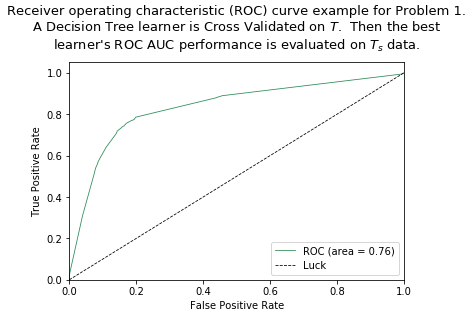
\includegraphics[width=1.2\columnwidth]{figures/figure-highROCAUC/figure-highROCAUC}
\caption{Example of a ROC curve from a Decision Tree classifier used on \cref{target1}. A 8-fold CV procedure is fit and then the best learner's performance is evaluated on $\mathcal{T_s}$ which gives score of $0.76$.}
\label{fg:highROCAUC}
\end{center}
\end{figure}


\subsection{Final experiments on models selection}\label{sub:final_model_selection}

As a last remark for this chapter, we show here a brief experiment with a Logistic Regression Classifier. Where we explore different hyperparameter configurations over a full CV procedure.

To do this, we set up to find users that lived in endemic regions in the past, namely \cref{target1}, yet excluding the feature that indicates in which state is the user currently living.
We also set the ``ROC AUC'' metric to compare the $l1$ vs the $l2$ regularization of the model on more than a hundred values for the regularization parameter $C$.

For both regularization types, we set a value for $C$ that ranged from $\exp^{-2}$ to $\exp^{5}$. Over all, we implement a cross validation routine was done on a training set with 8-folds.
.
\cref{tab:roc_auc_logreg_target1_results} shows a summary of results.
In these, our experiments resulted in higher values for $l1$ regularized models.
This gap is even widened when comparing test scores for both and the same happens to the time taken to fit the cross validation algorithm for all of the $C$ values.


\begin{table}[!htb]
\caption{Table of results comparing an 8 fold cross validation fit for a Logistic Classifier with varying regularization $C$ values.
The metric for this experiment was the ``ROC AUC'' and the \cref{target1} was tackled.}
\label{tab:roc_auc_logreg_target1_results}
\centering
\begin{tabular*}{0.9\textwidth}{@{\extracolsep{\fill} }  l l l l l }
%{|p{2cm}|p{2cm}|p{1.5cm}|p{1cm}|p{1.5cm}}
\toprule
Regularization type & Best CV $C$ value & Mean CV score & Test score & Full CV time (s)  \\
\midrule
$l2$ & 1e-5 & 0.805 & 0.744 & 17579.7  \\
$l1$ & 1e-5 & 0.81 & 0.76 & 15892.9 \\

\bottomrule
\end{tabular*}
\end{table}


Another interesting result is that in both experiments, the best CV scores were achieved for highly regularized models.
To further explore this, we looked at their CV mean scores for each hyperparameter setting.
\cref{fig:rocauc_logreg_cv_l1_regularized_comparison, rocauc_logreg_cv_l2_regularized_comparison} shows both series to compare.
 
 From these it is clear that both models improve the more regularized they become.
 The full extent to which this regularization would keep improving the score is not explored because both experiments' $C$ parameter had a minimum at $10^{-5}$ which corresponds to the highest score for both.
 Also, there is a difference in the stability of the fitting, where the scores are more noisy for the $l2$ regularization at high $C$ values as can be seen in \cref{rocauc_logreg_cv_l2_regularized_comparison}.

 On the other hand, the $l1$ regularization has a more stable performance across $C$.
 This can be an indication that the $l1$ experiment required less iterations to fit and find an optimum.

\begin{figure}[h!]
	\begin{center}
		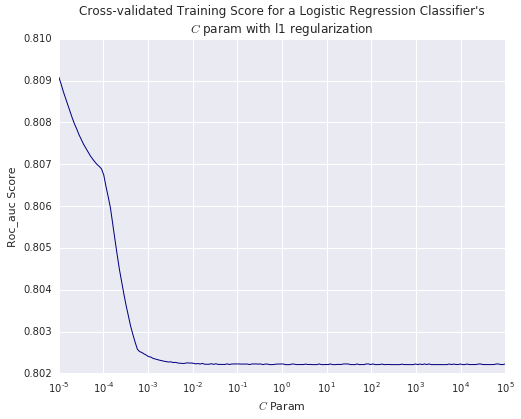
\includegraphics[width=0.7\linewidth]{figures/cross_validation/logreg_cv_regularization_l1_rocauc_series}
		\caption{Series of CV mean average scores for the ``ROC AUC'' metric where the $l1$ regularization method on a logistic classifier was tested, varying along the $C$ hyperparameter. 
			Here the \cref{target1} is tackled.}
		\label{fig:rocauc_logreg_cv_l1_regularized_comparison}
	\end{center}
\end{figure}



\begin{figure}[h!]
	\begin{center}
		 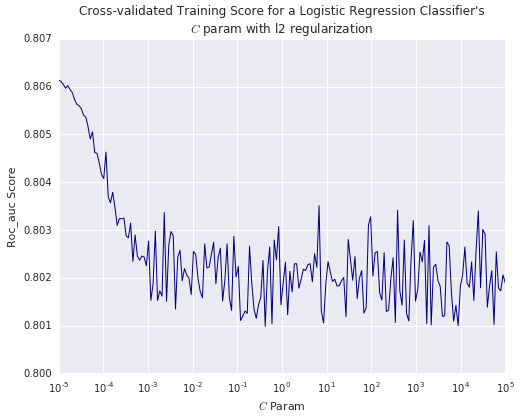
\includegraphics[width=0.7\linewidth]{figures/cross_validation/logreg_cv_regularization_l2_rocauc_series}
		\caption{Series of CV mean average scores for the ``ROC AUC'' metric where the $l2$ regularization method on a logistic classifier was tested, varying along the $C$ hyperparameter. 
			Here the \cref{target1} is tackled.}
		\label{fig:rocauc_logreg_cv_l2_regularized_comparison}
	\end{center}
\end{figure}


With these experiments we can have an extended overview of how a complete model selection pipeline works. Where we have to iterate and evaluate different hyper-parameter configurations by scoring the cross-validated learners.	